本文中的问题一，已通过查阅论文断定男胎 Y 染色体浓度与年龄无关。且本文已通过式 \ref{eq:final_model} 拟合出男胎 Y 染色体浓度与孕周、BMI 之间的关系，于问题二的基础上，本文继续综合考虑 BMI（由于共线性，不考虑将体重与身高纳入模型）、检测误差、胎儿的 Y 染色体浓度达标比例等因素，新增了多个约束条件。

\subsection{数据预分析}

该图展示了在不同Y染色体浓度区间内，检测结果为“准确”的样本所占的比例。为保证统计稳健性，图中仅包含样本数大于$10$的区间。从图中可以清晰地观察到：当浓度低于$4\%$时，检测准确率显著下降；而当浓度高于$4\%$后，准确样本的比例提升并维持在较高水平。

为探究检测误差与Y染色体浓度的内在联系，并为优化模型构建更稳健的约束条件，本文绘制了准确样本比例随Y染色体浓度变化的分布图（如图 \ref{fig:Y染色体浓度与预测准确的关系} 所示）。

\begin{figure} [H]
    \centering
    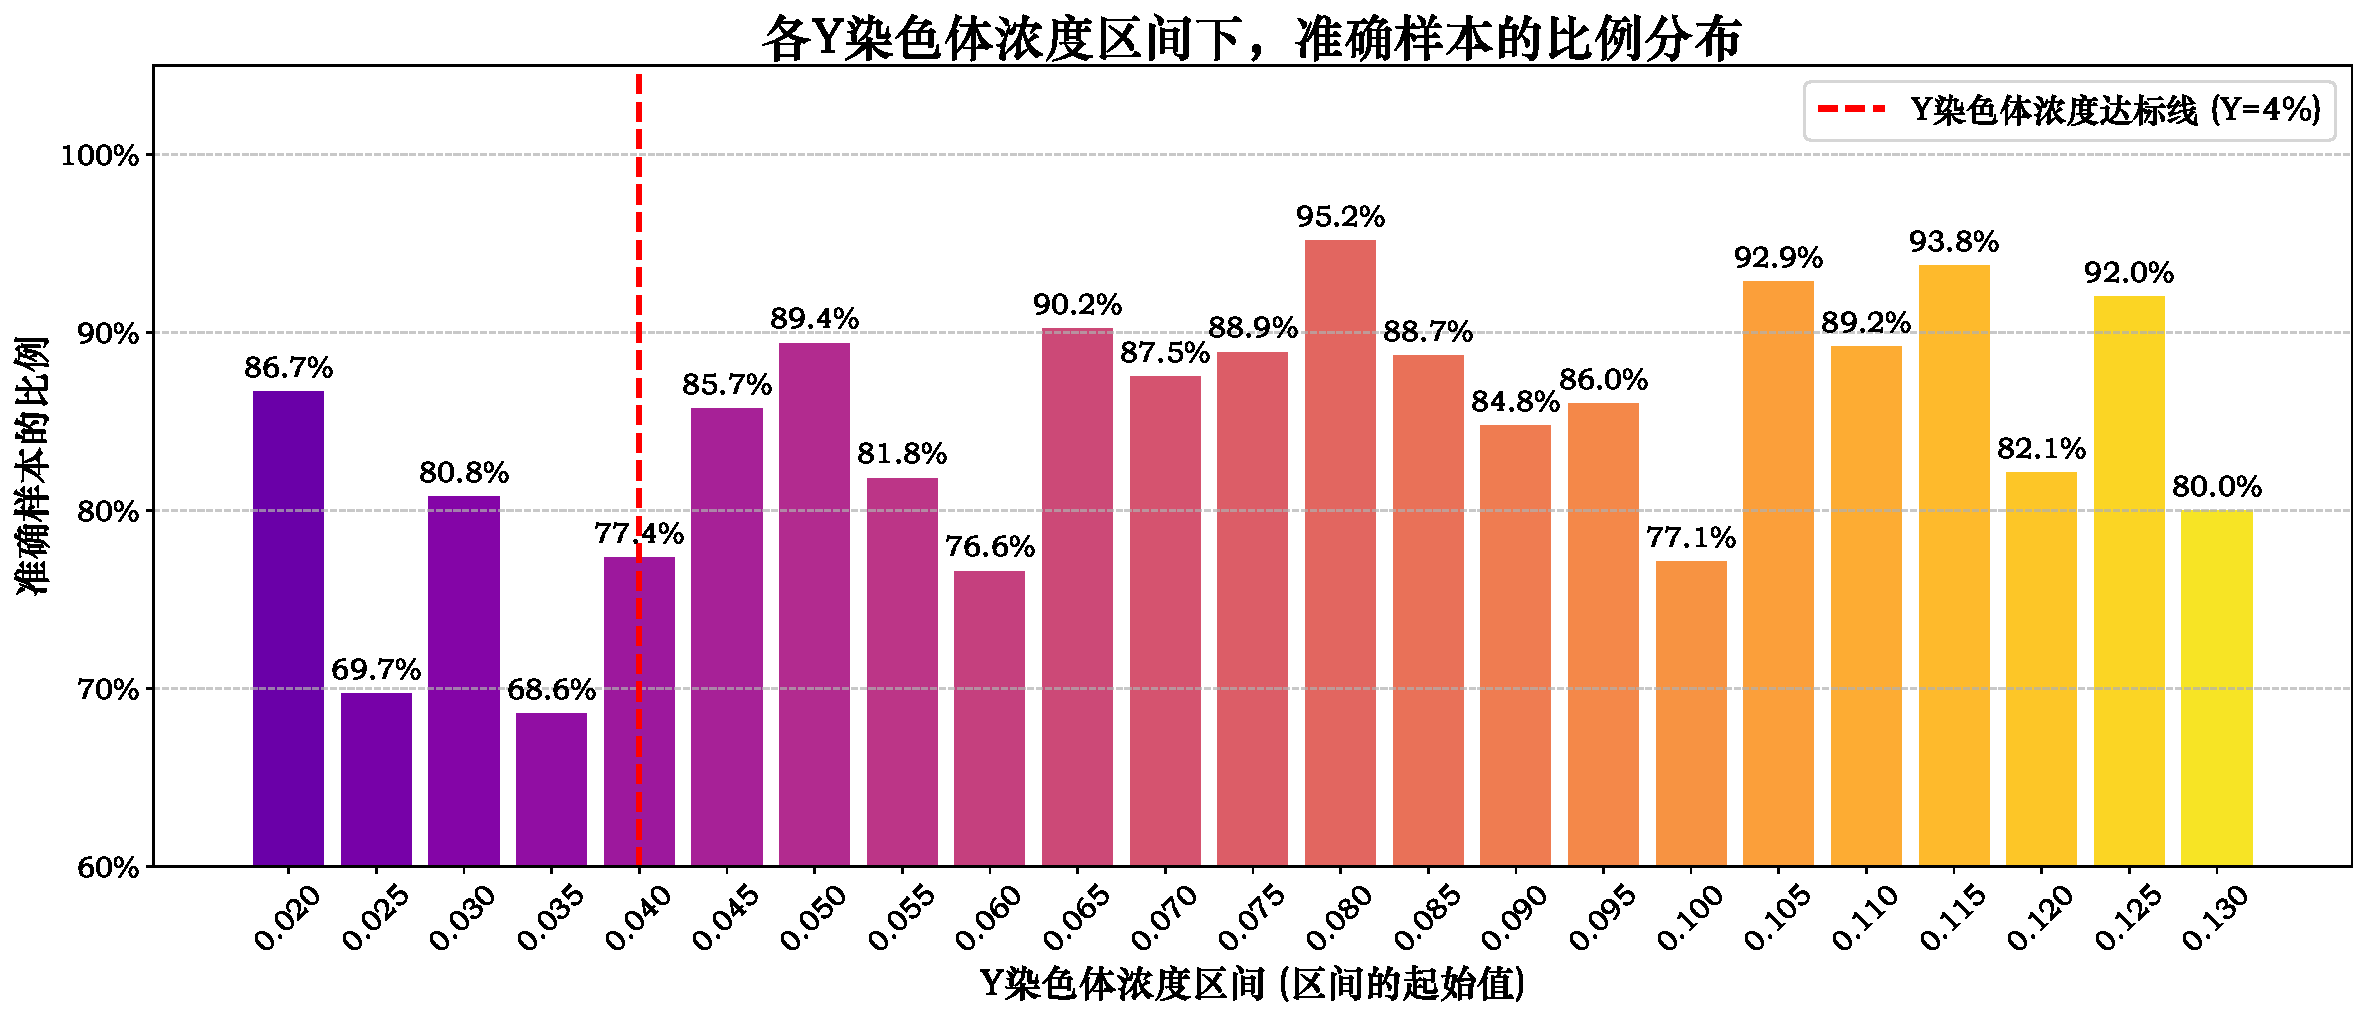
\includegraphics[width=0.8\textwidth]{chapters/Q3/images/Y染色体浓度与预测准确的关系.pdf}
    \caption{Y 染色体浓度与预测准确的关系}
    \label{fig:Y染色体浓度与预测准确的关系}
\end{figure}

\subsection{符号说明}

\begin{center}
    \begin{tabularx}{0.8\textwidth}{c@{\hspace{1pc}}|@{\hspace{2pc}}>{\centering\arraybackslash}X}
        \Xhline{0.08em} % 表格顶部粗线
        \textbf{符号}              & \textbf{符号说明（其余符号沿用上文符号）}               \\
        \Xhline{0.05em}
        $G_j$                    & 由边界点 $b_j$ 和 $b_{j+1}$ 定义的第 $j$ 个BMI分组。 \\
        $\hat{Y}(w, \text{bmi})$ & 根据第一问模型预测的Y染色体浓度。                       \\
        $P_{Y>6\%}(S_{j,w})$     & 窗口 $S_{j,w}$ 内Y染色体浓度大于6\%的样本比例。         \\
        \Xhline{0.08em}
    \end{tabularx}
\end{center}

\subsection{建立优化问题}

\subsubsection{目标函数}

此处，目标函数与问题二保持一致，参考式 \ref{eq:objective_function_final}.

\subsubsection{核心约束}

在$4\% \sim 6\%$的浓度区间内，准确率仍存在小幅波动，考虑到本文在问题一中所建立的预测模型 (\(Y = f(w, \text{BMI}, c)\)) 预测的是 Y 染色体浓度的数学期望，而任何临床单次测量的真实值都会围绕该均值存在随机波动。为规避随机波动的风险，且
基于图 \ref{fig:Y染色体浓度与预测准确的关系} 的数据，当Y染色体浓度超过$6\%$后，检测准确样本的比例更大。因此，本文构建如下约束条件，要求模型为各 BMI 分组推荐的最佳 NIPT 时点预测的 Y 染色体浓度理论值不低于$6\%$。
\begin{equation}
    \text{Y}_{ij} = f(w_{ij}^*, \text{BMI}_{ij}, c=1) \ge 0.06 \quad \forall j \in \{1, 2, 3, 4\}
    \label{eq:constraint_y_gt_6_percent}
\end{equation}
其中 $Y_{ij}$ 是第 $j$ 个分组中的第 $i$ 个孕妇在最佳孕周 $w_{ij}^*$ 时点的预测 Y 染色体浓度。

\subsubsection{软约束}

如果对于某个分组 $G_j$，在所有可能的孕周中都找不到任何一个能同时满足上述4个严格逻辑约束的窗口，模型会进入“宽松搜索”模式，只要求满足\textbf{窗口样本量约束}。然而，此时目标函数中的\textbf{惩罚项 $P(B)$}会被触发，其值会显著增大。这是一种软约束机制，它允许算法在找不到完美解时给出一个次优解，但会通过高昂的“罚分”来表明该解的质量有所欠缺，并激励算法继续寻找能满足所有严格约束的更优解。

\subsubsection{硬约束}

这些约束在优化过程中必须被严格满足。

\begin{enumerate}
    \item \textbf{边界点取值范围}: 所有BMI边界点 $b_i$ 必须位于数据集中BMI的最小值和最大值之间。
          \begin{equation}
              BMI_{\min} \le b_i \le BMI_{\max}, \quad \forall i \in \{1, \dots, 5\}
          \end{equation}

    \item \textbf{BMI分组最小宽度}: 为了避免产生过于狭窄、失去统计意义的分组，任意相邻两个边界点之间的差值必须不小于2.5。
          \begin{equation}
              |b_{i+1} - b_i| \ge 2.5, \quad \forall i \in \{1, \dots, 4\}
          \end{equation}
\end{enumerate}

\subsubsection{逻辑约束}

在目标函数内部，为每个给定的BMI分组 $G_j$ 寻找最佳孕周 $w_j^*$ 时，采用一个“严格-宽松”两阶段搜索策略。一个孕周窗口 $w_j$ 不仅要满足问题一的窗口长度，还必须满足以下\textbf{严格约束}，才被认为是理想的候选窗口：
\begin{enumerate}
    \item \textbf{窗口样本量}: 窗口内的样本数量 $N_{j,w}$ 必须在设定的范围内，以保证统计可靠性。
          \begin{equation}
              20 \le N_{j,w} \le 100
          \end{equation}
    \item \textbf{高Y浓度样本比例}: 窗口内，Y染色体浓度大于6\%的样本占比必须超过50\%，以确保窗口内的样本质量。
          \begin{equation}
              P_{Y>6\%}(S_{j,w}) \ge 0.50
          \end{equation}
\end{enumerate}

\subsection{差分进化求解}

本模型采用\textbf{差分进化}算法进行求解。差分算法是一种智能的启发式随机搜索算法，属于遗传算法的一种。它通过模拟生物进化过程中的变异、交叉和选择操作，在解空间中进行全局搜索。本文目标函数 $F(B)$ 依赖于对数据子集的复杂查询和搜索，且形态复杂（存在多个局部最优解）。对于这类问题，传统的梯度下降法难以奏效，而这样的全局优化算法则表现出色，能有效避免陷入局部最优，具有更强的鲁棒性。

我们通过调用 \texttt{scipy.optimize.differential\_evolution} 库函数来实现该算法。代码中设置了合理的种群大小（$popsize=30$）和最大迭代次数（$maxiter=100$），并启用了并行计算（$workers=4$）以加速收敛过程。经过差分进化算法优化求解，模型得到的最优BMI分组方案及对应的最佳 NIPT 时点建议如表 \ref{tab:q3_results} 所示。

\begin{table}[H]
    \centering
    \caption{最优BMI分组及NIPT时点推荐方案}
    \label{tab:q3_results}
    \begin{tabular}{cccc}
        \toprule
        \textbf{BMI分组} & \textbf{BMI区间} & \textbf{最佳NIPT时点 (周)} & \textbf{窗口内成功率} \\
        \midrule
        分组 1           & [29.07, 31.57) & 10 -- 12              & 80.00\%         \\
        分组 2           & [31.57, 34.11) & 11 -- 13              & 76.27\%         \\
        分组 3           & [34.11, 36.84) & 12 -- 14              & 77.78\%         \\
        分组 4           & [36.84, 43.07) & 23 -- 25              & 75.00\%         \\
        \bottomrule
    \end{tabular}
\end{table}

\v{-1em}

为直观验证该优化方案的有效性，本文将表 \ref{tab:q3_results} 中得到的四个最优NIPT推荐窗口，同样高亮矩形区域的形式叠加绘制在原始的散点图上，结果如图 \ref{fig:Q3_BMI分组和最佳NIPT时点} 所示 。从图中可以清晰地看出，模型推荐的窗口精确地覆盖了正常样本（蓝色点）的密集区域，同时有效规避了不准确样本（红色）和Y染色体浓度低于4\%的样本（橙色）的集中分布区。这直观地证实了模型在寻找最佳检测时点上的有效性。特别值得注意的是，对于BMI值最高的分组$4$（$BMI > 36.84$），模型推荐了一个明显更晚的检测窗口（$23 \sim 25$周），这与BMI越高、所需孕周越长的理论分析相符，进一步验证了模型的合理性。

\begin{figure}[H]
    \centering
    
\includegraphics[width=0.75\textwidth]{chapters/Q3/images/BMI分组和最佳NIPT时点.pdf}
    \caption{BMI分组和最佳NIPT时点}
    \label{fig:Q3_BMI分组和最佳NIPT时点}
\end{figure}

为进一步从数据层面评估本模型在规避检测误差方面的效果，本文采用了组内对比分析方法，将每个BMI分组在“推荐窗口”内的检测成功率与该组全体样本的“基线成功率”进行比较，对比结果如图 \ref{fig:Q3_组内检测成功率对比分析} 所示。

\begin{figure}[H]
    \centering
    
\includegraphics[width=0.8\textwidth]{chapters/Q3/images/组内检测成功率对比分析.pdf}
    \caption{组内检测成功率对比分析}
    \label{fig:Q3_组内检测成功率对比分析}
\end{figure}

\begin{itemize}
    \item 对于BMI较高的分组 $3$ 和分组 $4$，本模型计算所得的 NIPT 窗口极大地提升了检测成功率。分组 $3$ 的成功率从基线 $69.27\%$ 提升至 $77.78\%$ ，分组 $4$ 的成功率更是从 $60.29\%$ 大幅提升至 $75.00\%$。这表明对于高BMI这一高风险群体，本模型能有效定位到可显著降低检测失败风险的“黄金窗口”。
    \item 对于分组 $1$ 和分组 $2$，推荐窗口的成功率与基线水平相当（分组 $1$：$80.00\%$ VS $80.46\%$；分组 $2$：$76.27\%$ VS $76.97\%$）。这并非模型失效，而是多目标优化的必然结果。对于中低BMI的孕妇，可选的优质检测窗口较多，模型在保证高成功率的同时，会倾向于选择孕周更早的窗口以降低潜在风险。
\end{itemize}

综上所述，无论是从最优窗口的可视化定位，还是从组内成功率的量化对比来看，本文构建的模型及其求解结果都表现出良好的有效性和稳健性。它不仅能为不同BMI水平的孕妇群体提供定制化的 NIPT 时点建议，更能通过智能权衡，显著提升高风险群体的检测成功率，从而有效规避检测误差。